\documentclass[crop,tikz]{standalone}

\usepackage[utf8]{inputenc}

% 'crop' is the default for v1.0, before it was 'preview'
%\usetikzlibrary{...}% tikz package already loaded by 'tikz' option
\usetikzlibrary{arrows} 

\usetikzlibrary{decorations.markings}

\begin{document}

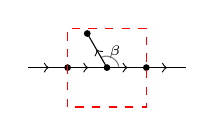
\begin{tikzpicture}%[->,>=stealth',auto,node distance=3cm,thick,main node/.style={circle,draw,font=\sffamily\Large\bfseries}]

	\draw[gray] (0.65,0) to[in=30, out=90] (0.5-0.075,0.866*0.15);
	\node[] at (0.6,0.2) {\tiny $\beta$};

	\begin{scope}[decoration={markings, mark=at position 0.525 with {\arrow{>}}}]
		\draw[postaction={decorate}] (-0.5,0) to (0,0);
		\draw[postaction={decorate}] (0,0) to (0.5,0);
		\draw[postaction={decorate}] (0.5,0) to (1,0);
		\draw[postaction={decorate}] (1,0) to (1.5,0);
		\draw[postaction={decorate}] (0.5,0) to (0.5-0.25, 0+0.433);
	\end{scope}	
	
	\filldraw[black] (0,0) circle (1pt); %node[anchor=east] {$v_1$};
	\filldraw[black] (1,0) circle (1pt); %node[anchor=west] {$v_2$};
	\filldraw[black] (0.5,0) circle (1pt);
	\filldraw[black] (0.5-0.25, 0+0.433) circle (1pt);
	
	\draw[dashed, red] (0,-0.5) rectangle (1,0.5);
	


\end{tikzpicture}

\end{document}